\begin{IEEEbiography}[{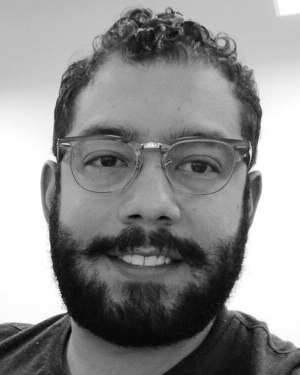
\includegraphics[width=1in,height=1.25in,clip,keepaspectratio]{../biography/yarib_300_375.jpg}}]{Yarib Nevarez} received the B.E. (Hons) degree in electronics from the Durango Institute of Technology, Durango, Mexico, in 2009, and the M.Sc. degree in Embedded Systems Design from the University of Applied Sciences Bremerhaven, Bremen, Germany, in 2017. He is currently pursuing a Ph.D. degree with the Institute of Electrodynamics and Microelectronics, University of Bremen, Germany. His research interest is focused mainly on System-on-Chip architectures and hardware implementation for deep learning accelerators in Embedded Systems.
\\
During his professional experience, he served as a Senior Embedded Software Engineer at Texas Instruments, IBM, Continental Automotive, TOSHIBA, and Carbon Robotics. He has designed and developed software architectures for graphic calculators, automotive systems, robotic drivers, and more.
	
\end{IEEEbiography}

\begin{IEEEbiography}[{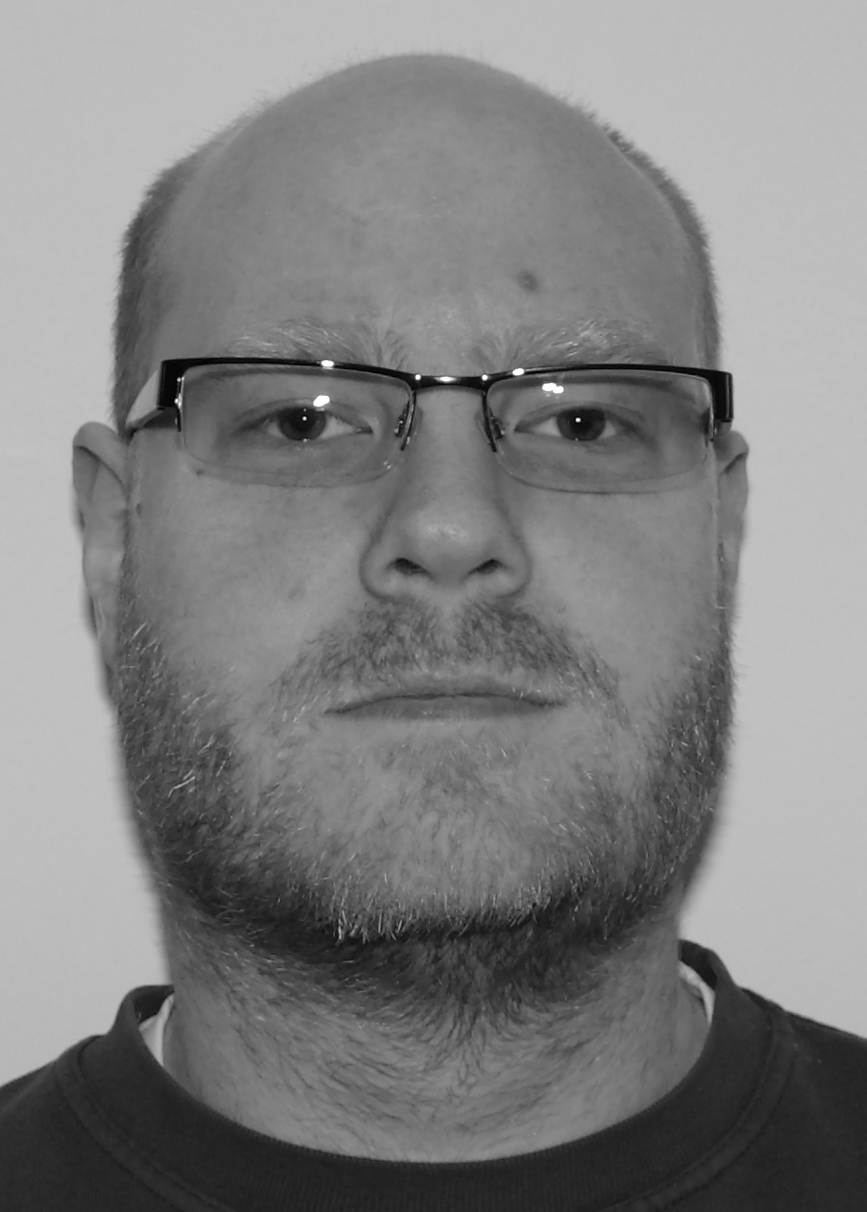
\includegraphics[width=1in,height=1.25in,clip,keepaspectratio]{../biography/Rotermund_David.jpg}}]{David Rotermund} started his scientific career as a chemical technical assistant in 1992 and received a pre-diploma in electrical engineering at the Hochschule Bremen (City University for Applied Science) in 1996. In 2002, he finished his studies of physics at the University of Bremen with a diploma (specialization in neuroscience and solid state physics). In 2007 he received his PhD "Extraction of information from the dynamical activities of neural networks". Among other neuroscience projects, he participated in several project in the field of neuro-prosthetics like the German-Israeli joint project "Models and Experiments towards Adaptive Control of Motor Prostheses" (METACOMP), the research focus Neurotechnology at the University of Bremen, and the Creative Unit "I-See: The artificial eye -- chronic wireless interface to the visual cortex". In the BMBF project KALOMED, where the goal was to design a fully wireless recording system that can be implanted under the skull of an user, he worked as project organizer and hardware/ software/ firmware designer as well as data miner. He will be the co-organizer of the upcoming Era-Net Neuron (a joint Canadian / EU project) for the development of advanced techniques in the field of visual cortex prosthesis. Beside his research in the field of neuro-prosthetics, he is keenly interested in information processing using spiking neuronal networks.
\end{IEEEbiography}

\begin{IEEEbiography}[{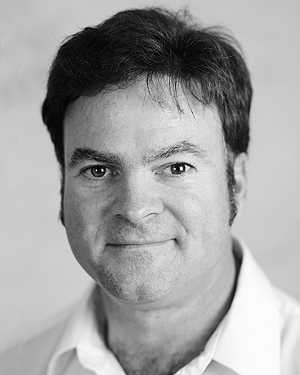
\includegraphics[width=1in,height=1.25in,clip,keepaspectratio]{../biography/klaus.png}}]{Klaus R. Pawelzik}
\end{IEEEbiography}

\begin{IEEEbiography}[{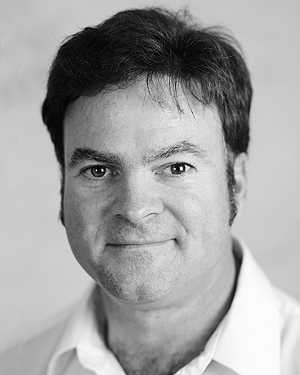
\includegraphics[width=1in,height=1.25in,clip,keepaspectratio]{../biography/alberto.png}}]{Alberto Garcia-Ortiz}
\end{IEEEbiography}
